% !TeX encoding = UTF-8
% !TeX spellcheck = en_US
% !TeX root = main.tex

\documentclass[11pt,oneside,a4paper]{memoir}

% General
\usepackage[utf8]{inputenc}
\usepackage[shorthands=off,english]{babel}
\usepackage{hyperref}
\usepackage{titlesec} 
\usepackage[noabbrev]{cleveref}
\usepackage[acronym,xindy,toc]{glossaries}

% Maths
\usepackage{amsmath}
\usepackage{amsfonts} % caligraphic fonts
\usepackage{amssymb}  % symbols
\usepackage{empheq}   % frame equations
\usepackage{siunitx}  % correct units

% Pictures
\usepackage{graphicx}
\usepackage{rotating}
\usepackage{epstopdf}
\usepackage{tikz}
\usetikzlibrary{shapes,arrows}

% Default fixed font does  support bold face

% Custom colors
\usepackage{color}
\definecolor{deepblue}{rgb}{0,0,0.5}
\definecolor{deepred}{rgb}{0.6,0,0}
\definecolor{deepgreen}{rgb}{0,0.5,0}
\definecolor{gray}{rgb}{0.5,0.5,0.4}

\usepackage{listings}
\usepackage{lstautogobble}
\renewcommand{\lstlistingname}{Code example}

% Python style for highlighting
\newcommand\pythonstyle{\lstset{
    language=Python,
    basicstyle=\linespread{1}\footnotesize\ttfamily,
    otherkeywords={self},             % Add keywords here
    keywordstyle=\footnotesize\ttfamily\bfseries\color{deepblue},
    emph={MyClass,__init__},          % Custom highlighting
    emphstyle=\bf\color{deepred},    % Custom highlighting style
    stringstyle=\color{deepgreen},
    frame=tb,                         % Any extra options here
    showstringspaces=false,           % 
    tabsize=4,
    numbers=left,    
    numberstyle=\tiny\color{gray}, 
    breaklines=true,
    autogobble=true,
    commentstyle=\color{gray},           
}}


% Python environment
\lstnewenvironment{python}[1][]
{
\pythonstyle
\lstset{#1}
}
{}

% Python for external files
\newcommand\pythonexternal[2][]{{
\pythonstyle
\lstinputlisting[#1]{#2}}}

\newcommand\cppstyle{\lstset{
    language=C++,
    basicstyle=\ttfamily,
    keywordstyle=\color{deepblue}\ttfamily,
    stringstyle=\color{red}\ttfamily,
    commentstyle=\color{grey}\ttfamily,
    morecomment=[l][\color{magenta}]{\#},
    autogobble=true,
}}

% C++ environment
\lstnewenvironment{c++}[1][]
{
    \cppstyle
    \lstset{#1}
}
{}

% % % % % % % % % % % % % % % % % %
% trick not to release comments   %
  \newif\ifrelease
%	                              %
	%\releasetrue
	\releasefalse
%	                              %
	\ifrelease
	\else
		\usepackage[colorinlistoftodos,textsize=scriptsize]{todonotes}
	\fi
% end of trick                    %
% % % % % % % % % % % % % % % % % %

\renewcommand{\vec}[1]{\underline{#1}}
\newcommand{\mat}[1]{\underline{\underline{#1}}}
\newcommand{\scal}[2]{\langle #1 {\,,\,} #2 \rangle}

\newcommand{\remark}{\paragraph{Remark ---}}
\setsecnumdepth{subsubsection}
%\maxtocdepth{subsection}
\renewcommand{\baselinestretch}{1.5} 
\setlrmarginsandblock{3cm}{2.5cm}{*}
\setulmarginsandblock{3cm}{2.5cm}{*}
\checkandfixthelayout

\def\thetitle{Localization and correction of orbit perturbations in BESSY II storage ring}
\def\thesubject{Master Thesis}
\def\theauthor{Olivier Churlaud}
\author{\theauthor}
\title{\thetitle}

\makeglossaries
\newacronym{bpm}{BPM}{Beam Position Monitor}

\hypersetup{
    unicode=true,
    pdftitle={\thetitle},
    pdfauthor={\theauthor},
    pdfsubject={\thesubject},
    colorlinks=true,       % false: boxed links; true: colored links
    linkcolor=teal,       % color of internal links (change box color with linkbordercolor)
    citecolor=olive,
    filecolor=red,
    urlcolor=blue
}

\begin{document}

\frontmatter
\clearpage
\thispagestyle{empty}
\maketitle
\vfill
\begin{abstract}
       ......
\end{abstract}
\vfill

\cleardoublepage
\tableofcontents*
\listoffigures*
\printglossaries
\mainmatter

\section{Background}
\label{sec:background}
\subsection{BESSY II}

\todo[inline]{Short history of BESSY II + some numbers = 1/2 page}
\subsection{Storage ring}
\todo[inline]{Purpose + Physics of the accelerator = 3-5 pages}
\subsection{Orbit and distortions}
\todo[inline]{Physics + examples = 1/2 - 1 pges}

% !TeX encoding = UTF-8
% !TeX spellcheck = en_US
% !TeX root = main.tex

\chapter{Basics of particle accelerator physics}
\label{sec:acc_physics}
In order to be able to localize and correct perturbation, the effects of a perturbation on a particle trajectory must be clearly understood. This section will the particle motion in circular accelerator and define the parameters needed for the following explanations.

The beam trajectory can be studied in various ways. One easier and well used method stems from the field of linear beam optics (by analogy between beam and light focusing and steering). Here will be solely described what is needed in the next sections. A full reference can be found in~\cite{book:wille}. This section is mostly inspired by the chapter 3 of this same reference.

\section{Geometry -- Frame of reference -- Kinematics}
The term \emph{orbit} refers to the ideal trajectory of the particles, which is fixed by the construction of the accelerator.

The frame of reference is $K=(\vec{e}_x,\vec{e}_y, \vec{e}_s)$, which origin follows the beam. $\vec{e}_x$ is the horizontal axis directed towards the exterior of the orbit and normal to its curve, $\vec{e}_y$ is the vertical axis and $\vec{e}_s$ the tangential axis to the orbit.
\begin{figure}
    \centering
    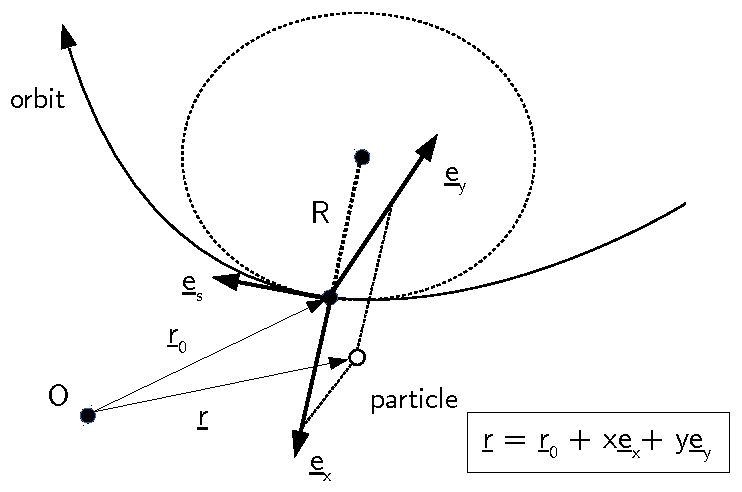
\includegraphics[width=0.8\linewidth]{img/orbit_coordinates.pdf}
    \caption[Description of the co-moving coordinate system]{\label{fig:coordinate system}Description of the co-moving coordinate system (inspired by~\cite{book:wille})}
\end{figure}
Let $\varphi$ be the azimuth angle, oriented by $\vec{e}_y$. Then, since $ds = -R d\varphi$, it can be writen
\begin{equation}
\frac{d \varphi}{d t}  = -\frac{1}{R} \frac{d s}{d t}.
\end{equation}

Using the derivation formula of polar coordinate yields
\begin{align}
&\dot{\vec{e}}_x = \frac{d\vec{e}_x}{d t} = -\dot{\varphi} \vec{e}_s = \frac{1}{R} \dot{s}\vec{e}_s \nonumber \\
&\dot{\vec{e}}_y = 0 \\
&\dot{\vec{e}}_s = \frac{d\vec{e}_s}{d t} = \dot{\varphi} \vec{e}_x = -\frac{1}{R} \dot{s}\vec{e}_x \nonumber.
\end{align}

Let $\vec{r} = \vec{r}_0 + x\vec{e}_x + y \vec{e}_y$ be the position of a given particle in a Galilean reference frame (with $\vec{r}_0$ the position of the origin of the moving coordinates, see \cref{fig:coordinate system}) and let $x'$ be the spatial derivative with respect to $s$ so that:
\begin{equation}
\begin{aligned}
&\dot{x}= \frac{dx}{ds}\frac{ds}{dt} = x'\dot{s}  \\
&\ddot{x}= x''\dot{s}^2+x'\ddot{s}.
\end{aligned}
\end{equation}
It follows, after some algebraic manipulations:
\begin{align}
\label{eq:kinematics}
&\vec{r} = \vec{r}_0 + x\vec{e}_x + y \vec{e}_y \nonumber \\
&\dot{\vec{r}}= x' \dot{s} \vec{e}_x + y'\dot{s} \vec{e}_y  + \left(1+\frac{x}{R}\right)\dot{s}\vec{e}_s\\
&\ddot{\vec{r}}= \left[x'' \dot{s}^2 + x' \ddot{s} - \left( 1+\frac{x}{R} \right)\frac{\dot{s}^2}{R}\right] \vec{e}_x + (y''\dot{s}^2 + y'\ddot{s}) \vec{e}_y \nonumber \\
& \hspace{14em} + \left[\frac{2}{R}x'\dot{s}^2 +\left(1+\frac{x}{R}\right)\ddot{s}\right]\vec{e}_s \nonumber
\end{align}

\section{Assumptions}
The following assumptions are assumed to be valid.
\begin{description}
    \item{A1 --} The particles move essentially parallel to $\vec{e}_s$: in the first order
    \begin{equation*}
        \vec{v} = v_s \vec{e}_s.
    \end{equation*}
    \item{A2 --} The magnetic field has only transverse components:
        \begin{equation*}
        \vec{B} = (B_x, B_y, 0).
        \end{equation*}
    \item{A3 --} The electric field is negligible with respect to the magnetic field.
    \item{A4 --} The velocity of the particle varies very slowly in a magnet: $\ddot{s} \approx 0$.
    \item{A5 --} The particles move at relativistic velocities, so the effect of the magnetic field is negligible on longitudinal components: only transverse components will be considered.
    \item{A6 --} The momentum of the particles is $p = p_0+\Delta p$, with the condition $\Delta p \ll p_0$ (which is well satisfied in accelerators).
\end{description}

\section{Equation of motion}
\label{sec:eq_motion}
Newton's second law can be applied with the Lorentz force
\begin{equation}
\dot{\vec{p}} = e(\vec{E}+\vec{v} \times \vec{B}) 
\end{equation}
which according to (A3) becomes
\begin{equation}
\ddot{\vec{r}} = \frac{e}{m}(\dot{\vec{r}} \times \vec{B})
\end{equation}

According to (A2), the magnetic field is only transversal, which yields
\begin{equation}
\label{eq:lorentz_transv}
\ddot{\vec{r}} = \frac{e}{m}(\dot{\vec{r}} \times \vec{B})
= \frac{e}{m}
    \begin{pmatrix}
        -\left(1+\frac{x}{R}\right)\dot{s}B_y \\
        \left(1+\frac{x}{R}\right)\dot{s}B_x \\
        x'\dot{s}B_y - y'\dot{s}B_x
    \end{pmatrix}.
\end{equation}

Using (A5), the $s$-component does not need to be considered and using (A4) in \cref{eq:kinematics} allows to remove every $\ddot{s}$ factors, so that \cref{eq:lorentz_transv} can be rewritten as
\begin{equation}
\begin{aligned}
x'' \dot{s}^2 - \left(1+\frac{x}{R}\right)\frac{\dot{s}^2}{R}
&= -\frac{e}{m} \left(1+\frac{x}{R}\right)\dot{s}B_y \\
y'' \dot{s}^2 &=    \left(1+\frac{x}{R}\right)\dot{s}B_x.
\end{aligned}
\end{equation}
Finally, because $p=mv$ and using \cref{eq:kinematics} combined with (A1),
\begin{equation}
m = \frac{p}{v} = \frac{p}{\scal{\vec{v}}{\vec{e}_s}} = \frac{p}{\left(1+\frac{x}{R}\right)\dot{s}}
\end{equation}
can be substituted to obtain
\begin{equation}
\begin{aligned}
x''-\left(1+\frac{x}{R}\right)\frac{1}{R} &= -\frac{e}{p} B_y\left(1+\frac{x}{R}\right)^2 \\
y'' &= \frac{e}{p} B_x\left(1+\frac{x}{R}\right)^2
\end{aligned}
\end{equation}

According to (A6), it can be written to first order
\begin{equation*}
\frac{1}{p} = \frac{1}{p_0} \left(1-\frac{\Delta p}{p_0}\right).
\end{equation*}

Furthermore the magnetic field can be approximated to first order with:
\begin{equation}
\frac{e}{p_0} B_y = \frac{1}{R}-kx \qquad\qquad \frac{e}{p_0} B_x = -ky
\end{equation}
which yields
\begin{equation}
\begin{aligned}
x''-\left(1+\frac{x}{R}\right)\frac{1}{R} &= -\left(\frac{1}{R}-kx\right)\left(1-\frac{\Delta p}{p_0}\right)\left(1+\frac{x}{R}\right)^2 \\
y'' &= -ky\left(1-\frac{\Delta p}{p_0}\right)\left(1+\frac{x}{R}\right)^2
\end{aligned}
\end{equation}

Finally removing terms of second order ($\frac{x}{R} \ll 1$, $\frac{\Delta p}{p_0} \ll 1$) leads to the linear equations of motion in a magnetic structure:

\begin{empheq}[box=\fbox]{equation}
\label{eq:motion_particle}
\begin{aligned}
x''(s) + \left(\frac{1}{R^2(s)} - k(s)\right) x(s) &= \frac{1}{R(s)}\frac{\Delta p}{p_0} \\
y''(s) + k(s) y(s) &= 0
\end{aligned}
\end{empheq}

\section{Beta function and betatron oscillation}
\label{sec:beta_func}
The beta function will provide a description of properties of a beam of many particles.

The only further assumption is that $\frac{1}{R} = 0$ and $\frac{\Delta p}{p_0}=0$. The orbit curve is thus assumed almost flat and the momentum deviation negligible. \Cref{eq:motion_particle} turns in Hill's differential equation: 
\begin{equation}
\label{eq:hill_diff}
	x''(s) - k(s) x(s) = 0
\end{equation}
which solution is the transverse oscillation of the orbit, or \emph{betatron oscillation}
\begin{equation}
\label{eq:hill_sol_cst}
x(s) = A u(s) \cos \left(\Psi(s)+\phi \right).
\end{equation}

The phase and the amplitude depend of the position $s$; $A$ and $\phi$ being integration constants.

Inserting \cref{eq:hill_sol_cst} in \eqref{eq:hill_diff} it follows
\begin{equation}
A\left[u''- u \Psi'^2 - k u \right] \cos\left(\Psi+\phi\right) - A\left[2u'\Psi'+u\Psi''\right]\sin\left(\Psi+\phi\right) = 0.
\end{equation}

$A \ne 0$ and $\Psi(s)$ having different values for every $s$, the previous equation provides two conditions
\begin{align}
u''- u \Psi'^2 - k u = 0 \label{eq:hill_cond1}\\
2u'\Psi'+u\Psi'' = 0 \label{eq:hill_cond2}.
\end{align}

\Cref{eq:hill_cond2} leads to
\begin{equation}
2\frac{u'}{u} + \frac{\Psi''}{\Psi'} = 0
\end{equation}
which can be integrated as
\begin{equation}
\label{eq:phase_psi}
\Psi(s) = \int \limits_{0}^{s} \frac{d\sigma}{u^2(\sigma)}.
\end{equation}

The \emph{beta function} $\beta(s)$ is defined as
\begin{equation}
\label{eq:beta_func}
\beta(s) := u^2(s).
\end{equation}

Substituting $A = \sqrt{\varepsilon}$ provides the final trajectory equation
\begin{empheq}[box=\fbox]{equation}
	\label{eq:orbit_equation}
	x(s) = \sqrt{\varepsilon \beta(s)} \cos\left(\Psi(s)+\phi \right)
\end{empheq}

The constant $\varepsilon$ is termed \emph{emittance} and the envelop of the orbit at each position $s$ is $E(s) = \sqrt{\varepsilon \beta(s)}$, which defines the size of the beam.

Since the beta function controls the size of the beam, this is the function that must be finely controlled. A matrix calculation method is presented in \cite{book:wille} in order to calculate it step by step around the orbit. Knowing this, $\Psi$ can be calculated by rewriting \cref{eq:phase_psi} as 
\begin{empheq}[box=\fbox]{equation}
\Psi(s)=\int \limits_{0}^{s} \frac{d\sigma}{\beta(\sigma)},
\end{empheq}
and the particle trajectories can be calculated for a given emittance.

Theses two functions $\Psi$ and $\beta$ will be extensively used in the next sections as the perturbation localization process and several correction methods rely on them.

\remark The calculation done for the $x$ direction can be done similarly for the $y$ one, which defines a $\beta_x(s)$, $\beta_y(s)$, $\varepsilon_x$, $\varepsilon_y$, $\Psi_x(s)$ and $\Psi_y(s)$

\section{Tune}
In circular accelerator, the particle undergo periodically the same magnetic fields and therefore the same force. This can lead the amplitude of the beam transverse oscillation to increase, risking to lose the particles in the vacuum chamber walls. This phenomenon is called optical resonance and must be avoided.

As exposed in \cref{sec:eq_motion,sec:beta_func}, if $\frac{\Delta p}{p_0} = 0$ and $K(s)=\frac{1}{R(s)}-k(s)$, the trajectory is given by
\begin{equation}
x''(s)+K(s) x(s) = 0.
\end{equation}

Since $K(s)$ is periodic with the circumference $L$ of the ring, then the trajectory is again (according to Floquet's theorem)
\begin{equation}
x(s) = \sqrt{\varepsilon \beta(s)} \cos\left(\Psi(s)+\Phi\right)
\end{equation}
with $\beta(s)$ periodic of period $L$ as well. The resonant behavior depending on the betatron phase $\Delta \Psi = \Psi(s+L)-\Psi(s)$, the tune $Q$ of the accelerator is defined as
\begin{equation}
\label{eq:tune}
Q = \frac{\Delta \Psi}{2 \pi} = \frac{1}{2 \pi} \oint\frac{ds}{\beta(s)}.
\end{equation}

The tune is a constant for a circular accelerator: it describes the number of betatron oscillation undergone by a particle per revolution.

It can be shown that tune values that satisfy 
\begin{equation}
\label{eq:coupled_resonance}
m Q_x + n Q_y = p \qquad (m, n, p) \in \mathbb{Z}
\end{equation}
produce coupled resonance of order $|m|+|n|$. A pair of value $(Q_x,Q_y)$ is used as working point so that it either does not satisfy \cref{eq:coupled_resonance} or with a high order (above the 5th order for instance).

\section{Summary}
Two very important functions were defined here: $\beta (s)$ and $\Psi (s)$, respectively the variation of the trajectory amplitude and the betatron phase. These functions highly depend on the accelerator optic and when determined, knowing the real objects that produce them (e.g. magnets, spools) is no more needed.

The tune $Q$ is a constant parameter defined from them as the number of betatron oscillation per revolution.

The following sections will rely on these three variables as they fully represent the orbit and its variations.
% !TeX encoding = UTF-8
% !TeX spellcheck = en_US
% !TeX root = main.tex

\chapter{Localization of orbit distortion}
\label{sec:localisation}

Correcting the orbit is costly and has never a perfect result. Instead of dealing with the effects, we can deal with the sources of the distortions. If none is really obvious (\textit{eg.} a non-isolated transformer, the 50~Hz perturbation of the main power), the orbit can give us some hints.

We call kick the place where the orbit brutally changes its angle as shown in Fig.~\ref{fig:kick}.

\begin{figure}[!h]
	\centering
	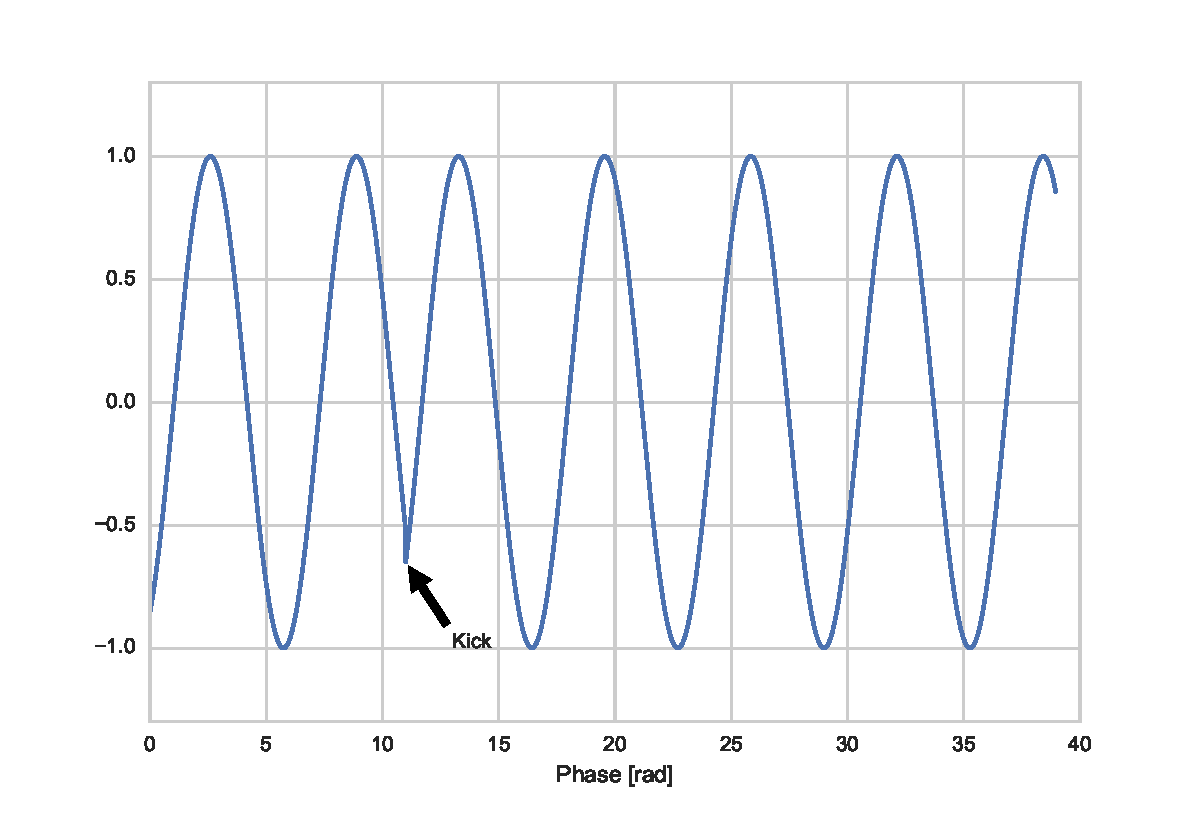
\includegraphics[width=.9\linewidth]{img/kick}
	\caption{\label{fig:kick}Example of kick in the orbit}
\end{figure}

\section{Theory}
\label{ssec:loc_theory}

\subsection{Theoretical setting of the problem}

Everything is described here with the phase variable $\phi = \int\limits_{0}^s \frac{d\sigma}{\beta(\sigma)}$. The spatial variable is only used to have a connection between the result and the actual ring. The explanation will be led with the $x$ variable, but is also valid with the $y$ one.

Let one kick be at $\phi = \hat{\phi}$. The orbit is modified and oscillates with a constant period of $2 \pi$. Because there is {\em only one} kick and according to the closed orbit condition, the oscillation after the kick will be stable for one revolution. Furthermore, the orbit must be continuous on all points, thus at the kick position too.

Let's consider two revolutions, in order to be sure to find one full revolution without kick. Let $\phi_\mathrm{ext} \in [0, 4 \pi Q]$ be this new phase (\textit{ext} for extended). The phase $\phi_0$ where the kick happens is the one so that 
\begin{equation}
\exists (b, c) \in \mathbb{R}^2:
\forall \phi \in [\phi_0, \phi_0 + 2 \pi Q], \quad
x(\phi) = b \sin(\phi + c)
\end{equation}

We have a problem with 3 unknowns to determine: $\phi_0, b, c$. 

\subsection{Practical setting}

We have $m$ BPMs only, distributed around the orbit.
Therefore we define:
\begin{align}
\begin{cases}
\vec{\phi} = [\phi_0, \phi_1, ..., \phi_{m-1}] \\
\vec{x} = [x_0, x_1, ..., x_{m-1}]
\end{cases} \quad \mathrm{and} \quad
\begin{cases}
\vec{\phi}_\mathrm{ext} = [\vec{\phi}, \vec{\phi}+2\pi Q ]\\
\vec{x}_\mathrm{ext} = [\vec{x}, \vec{x}]
\end{cases}
\end{align}

\subsection{Solving the problem}

To find the kick in the orbit it suffices to find a sine that fits in $\vec{x}_\mathrm{ext}$.

An algorithm is designed to find a sine over a revolution, beginning at each BPM and keep the one that fit at best:
\begin{align}
\forall k \in &[0, m-1], \nonumber \\
&\begin{cases}
\vec{\phi}^k = [\vec{\phi}_\mathrm{ext}(k), \vec{\phi}_\mathrm{ext}(k+1), \cdots,  \vec{\phi}_\mathrm{ext}(k+m-1)]\\
\vec{x}^k = [\vec{x}_\mathrm{ext}(k), \vec{x}_\mathrm{ext}(k+1), \cdots,  \vec{x}_\mathrm{ext}(k+m-1)]\\
\tilde{\vec{x}} = \mathtt{fit\_sine}(\vec{x}^k, \vec{\phi}^k)
\end{cases}
\end{align}

It is then defined

\begin{equation}
k_0 = \underset{k \in [0, m-1]}{\textrm{argmin}}\{||\tilde{\vec{x}}-\vec{x}^k||_2\}
\end{equation}

The kick is between $\phi_{k_0-1}$ and $\phi_{k_0+1}$, and we assume that the closest sine is $\tilde{x}(\phi) = b \sin(\phi + c) $.

To find the exact position of the kick, we use the property of closed orbit: the orbit must be continuous also at the kick phase, which means that $\hat{\phi}$ is the solution of
\begin{equation}
b \sin(\phi + c) = b\sin(\phi+c-2 \pi Q), \qquad \mathrm{with}~ \phi \in [\phi_{k_0-1}, \phi_{k_0+1}]
\end{equation}
or, with the numerical approach, 
\begin{equation}
\hat{\phi} =  \underset{\phi \in [\phi_{k_0-1}, \phi_{k_0+1}]}{\textrm{argmin}}\{|b \sin(\phi + c) - b\sin(\phi+c-2 \pi Q)|\}
\end{equation}

\remark For this last step, we use a \textit{linspace} between $\phi_{k_0-1}$ and $\phi_{k_0+1}$ with more than 1000 points.

\remark One should be careful if $k_0 = 0$ (resp. $k_0 = m-1$) and set $\phi_{k_0-1} =\phi_{m-1}$ (resp. $\phi_{k_0+1} = \phi_{0}$). 

\subsection{Finding the good sine}
Several methods are possible to find the best matching sine, for example by using:
\begin{itemize}
	\item a pseudo-inversion
	\item a scalar-product with a sine (resp. a cosine)
\end{itemize}

\paragraph{Pseudo-inversion}
The problem can be set as a linear equation problem as follow.
\begin{align}
&\forall k \in [0,m-1], \tilde{x}(\phi_k) = a_1 \cos(\phi_k) + a_2 \sin(\phi_k) + a \nonumber \\
%
\implies &
\begin{pmatrix}
1 & \cos(\phi_0) & \sin(\phi_0) \\
1 & \cos(\phi_1) & \sin(\phi_1) \\
\vdots & \vdots & \vdots \\
1 & \cos(\phi_{m-1}) & \sin(\phi_{m-1}) \\
\end{pmatrix}
\begin{pmatrix}
a \\ a_1 \\ a_2
\end{pmatrix}
=
\begin{pmatrix}
x_0 \\ x_2 \\ \vdots \\ x_{m-1}
\end{pmatrix} \nonumber
\\
%
\implies &
\begin{pmatrix}
a \\ a_1 \\ a_2
\end{pmatrix}
= 
\mathrm{pseudo\_inv}
\begin{pmatrix}
1 & \cos(\phi_0) & \sin(\phi_0) \\
1 & \cos(\phi_1) & \sin(\phi_1) \\
\vdots & \vdots & \vdots \\
1 & \cos(\phi_{m-1}) & \sin(\phi_{m-1}) \\
\end{pmatrix}
\begin{pmatrix}
x_0 \\ x_2 \\ \vdots \\ x_{m-1}
\end{pmatrix}
\end{align}

The pseudo inverse is calculated in \texttt{Matlab} with \verb$a = M\x$ and in \texttt{python} with \verb$a = numpy.linalg.lstsq(M, x)$ (least-squares solution).

\paragraph{Scalar product with a sine (resp. cosine)}
Since the orbit is expected to be written as
\begin{equation*}
x(\phi) = a_1 \cos(\phi) + a_2 \sin(\phi) + a
\end{equation*}
we can also describe it as
\begin{equation}
x(\phi) = \scal{x}{\cos} \cos(\phi) + \scal{x}{\sin} \sin(\phi) + \scal{x}{1}
\end{equation}
with $\scal{f}{g}$ being the scalar product for real functions: $\int_T f(t)g(u)dt$.

In our numerical case, we approximate this scalar product by its vectorial counterpart by:

\begin{align*}
\scal{\vec{f}}{\vec{g}}: \quad
 &\mathcal{R}^n \times \mathcal{R}^n \longrightarrow \mathcal{R} \\
 & (\vec{f},\vec{g}) \quad\longmapsto \quad \frac{1}{n}\sum\limits_{k=0}^{n-1} f_i g_i
\end{align*}

\paragraph{Coefficient format}
By defining $b = \sqrt{a_1^2+a_2^2}$ and $c = \mathrm{atan2}(a_1, a_2)$  we can write

\begin{equation*}
\tilde{x}(\phi) = a + a_1 \cos(\phi) + a_2 \sin(\phi) = a + b \sin(\phi + c).
\end{equation*} 

\section{Applications}
\todo[inline]{NOT UPDATED: DO NOT CORRECT THIS}
\subsection{Getting the position of a perturbation at a given frequency}
In this section, we deal with a perturbation at a given frequency $f$. The training data is the time signal of all BPMs.

As the perturbation has a known frequency, we extract its complex amplitude from the signal of each BPM with a Fourier transform:

\begin{equation}
\forall i \in [1, \mathrm{BPM\_nb}], \qquad 
\begin{cases}
\vec{X}_i = \mathrm{FFT}(\vec{x}_i) \\
c_i = \vec{X}_i(f)
\end{cases}
\end{equation}

\paragraph{Case of a unique perturbation source}

If the perturbation is unique, then all complex amplitude exactly describe the same sine of frequency $f$ and phase $\alpha_0$. It allows us to describe the complex vector $\vec{c}$ with $\vec{\hat{c}}$, which is real.

\begin{align}
&\alpha_0 = \underset{\alpha \in [0, 2\pi]}{\textrm{argmin}}\{\mathcal{R}e (\vec{c} \cdot e^{-j\alpha}) \} \\
&\vec{\hat{c}} = \mathcal{I}m (\vec{c} \cdot e^{-j\alpha_0})
\end{align}

The new signal $\vec{\hat{c}}$ can be used as an orbit signal: we have one orbit amplitude for each BPM: the kick can be extracted from it with the previous method described in Section \ref{ssec:loc_theory}.


\paragraph{Case of several perturbation sources}
If there are several perturbation sources, a $\alpha_0$ that let the cosine part vanish cannot be found. 


\section{Implementation}
\begin{python}[caption=Get the kick]
	import matplotlib.plt as plt
	import search_kick.core as skcore
	
	# Dataset
	orbit = ..
	phase = ..
	tune = ..
	
	# Get the kick and rebuild the ideal sine
	kick_phase, sin_coef = skcore.get_kick(orbit, phase, tune)
	sine, phase_th = skcore.build_sine(kick_phase, tune, sin_coef)
	
	# Plot the results
	plt.plot(phase, orbit, '-b')
	plt.plot(phase_th, sine, '-g')
	plt.axvline(kick, -2, 2)	
\end{python}


\section{Examples}


% !TeX encoding = UTF-8
% !TeX spellcheck = en_US
% !TeX root = main.tex
\tikzset{
	block/.style = {draw, fill=white, rectangle, minimum height=3em, minimum width=4em},
	gain/.style = {draw, fill=white, isosceles triangle, minimum height=3em, minimum width=2em},
	operator/.style= {draw, fill=white, circle},
	input/.style = {coordinate},
	output/.style= {coordinate},
	pinstyle/.style = {pin edge={to-,thin,black}},
}

\chapter{Orbit correction}
\label{sec:correction}

\section{Motivation}
The accelerators are designed so that the particles follow a given path, which is defined in the case of synchrotrons by the successive bendings involved by the magnets. As the precision of the positioning of the magnets is limited, some errors may destabilize the orbit and increase the dispersion of the particles around the theoretical orbit. In addition, the environment produces perturbations: for instance the 50~Hz of the main power, some not perfectly isolated magnetic sources.

In order not to lose electrons in the walls of the vacuum chamber but also to increase the brightness of the synchrotron radiations (and therefore to have focused electron beams), all these residual misalignment and magnetic field errors must be corrected.

\section{Some documented methods}
Several global corrections methods are well documented in the literature. The most common ones are the best corrector method and the response matrix method (see \cref{sec:most_effective_corr,sec:response_matrix}). 

Local orbit bumps (presented in \cref{sec:orbit_bump}) allow local correction and are used to change the path of the orbit (during the injection time for example).

\subsection{Local orbit bumps}
\label{sec:orbit_bump}
\begin{figure}
	\centering
	\begin{tikzpicture}[auto, node distance=1.2,>=latex']
	%\draw[help lines, yellow] (-1,-4)grid(15,3);
	% We start by placing the blocks
	\coordinate [] (lleft) {};
	\node [draw, circle, fill=black, right=2 of lleft] (leftm) {};
	\node [draw, circle, fill=black, above right=2 and 2.5 of leftm] (topm) {};
	\node [draw, circle, fill=black, right=5 of leftm] (rightm) {};
	\coordinate [right=2 of rightm] (rright) {};
	% Once the nodes are placed, connecting them is easy. 
	\draw [-] (lleft) -- node {}(leftm);
	\draw [-] (leftm) -- node {}(topm);
	\draw [-] (topm) -- node {}(rightm);
	\draw [-] (rightm) -- node {}(rright);
	\end{tikzpicture}
	\caption{\label{fig:local_bump}Local bump with 3 magnets}
\end{figure}
\todo[inline]{see Wille p127 and p286}

\subsection{Most effective corrector method}
\label{sec:most_effective_corr}
This method is based on the fact that orbit shifts are often caused by strong localized disturbances. Its goal is to correct particularly each disturbance.

\subsubsection{Principle}

Given a distorted orbit, the optimal gain for each corrector is calculated by a mean square error algorithm (see \cref{eq:gain_bestcorr} and \cite{book:wille}). The corrector which provides the best correction is selected: it is the most effective corrector.

Let's assume that the $i$th corrector, at position $s_i$, has the optical parameters $\beta_i$, $\alpha_i$ and $\Psi_i$, and that $m$ monitors are set around the orbit with parameters $\beta_j$, $\alpha_j$ and $\Psi_j$, and read a displacement $u_j$ from the reference orbit ($1 \leq j \leq m$).

The strength $\kappa_i$ of the field at the position $s_i$ is obtained minimizing the function
\todo{Explain in chap 1.3}
\begin{equation}
    \label{eq:gain_bestcorr}
    f_i(\kappa_i) = \sum\limits_{j=1}^{m} (u_j-x_{ij}(\kappa_i))^2 
                  = \sum\limits_{j=1}^{m} (u_j- \kappa_i h_{ij})^2
\end{equation}

with, if $\Delta \Psi_{ij} := \Psi_j-\Psi_i$,

\begin{align}
    \label{eq:hij}
    x_{ij}(\kappa_i) &= \kappa_i h_{ij} \nonumber\\
                     &= \kappa_i \frac{\sqrt{\beta_i \beta_j}}{2}
                         \left[
                             \frac{\cos(\Delta \Psi_{ij}) - 2\alpha_i \sin(\Delta\Psi_{ij})}
                                  {\tan (\pi Q)} + \sin (\Delta\Psi_{ij})
                         \right].
\end{align}

It follows that 
\begin{equation}
    \kappa_i = \frac{\sum\limits_{j=1}^m u_j h_{ij}}{\sum\limits_{j=1}^m h_{ij}^2}
\end{equation}

The $i$th corrector is attributed the gain $-\kappa_i$ to compensate the field.

\subsubsection{Iterative version}
When the most effective corrector is found, the process is reiterated on the corrected orbit with the remaining correctors. By doing this until all corrector are used (or that adding a correction does not improve the orbit) a comprehensive correction is reached.

\subsubsection{Practical issue}
The problem of this method is that each corrector must be tested once, and this for each iteration: the initialization of the correction is long and is then fixed. Moreover, the correction is less efficient than the other ones presented here~\cite{book:wille}.

\subsection{Inversion of the response matrix}
\label{sec:response_matrix}
This section is mainly based on~\cite{book:wille}, \cite{art:decker-1991} and \cite{art:plouviez-1999}.

\subsubsection{Inverse problem}
This correction is based on solving the following inverse problem: the expected orbit being known, how to set the correctors in order to achieve it? To solve it, the response matrix $\mat{S}$ is introduced.

The response matrix $\mat{S}$ is defined by the equation $\vec{X} = \mat{S}\, \vec{\Theta}$ where $\vec{\Theta}$ is the \emph{kick vector} (i.e. the vector of strength of the field generated by each corrector) and $\vec{X}$ the vector of \emph{orbit change}. If the accelerator has $M$ monitors and $N$ correctors, then $\mat{S}$ is a $M \times N$ matrix. $\mat{S}$ is often termed \emph{forward} or \emph{observation matrix} because it describes the effects of a given phenomenon. Indeed, each coefficient $S_{ij}$ of the matrix is the orbit change at the position $s_i$ (of the $i$th monitor), for a kick of unity 1 at the position $s_j$ (of the $j$th corrector).

Inversing the response matrix will provide the correction to apply. Since it's very common to have more monitors than correctors, the matrix is not square. A \emph{singular value decomposition} (SVD) is used on the matrix to provide a pseudo-inversion $\mat{S}^*$ of $\mat{S}$.

Using the SVD also allows to use only the most significant singular values in the correction. This prevents to over-correct the orbit, by not considering less significant values that can result of noise in the monitors during the measure, or numerical artifacts for instance.

The correction can then be performed
\begin{equation}
\vec{\Theta} = \mat{S}^* \vec{X}.
\end{equation}

\subsubsection{Acquisition of the response matrix}
Before solving the inverse problem, the response matrix must first be determined. This can be achieved in two different ways: by describing the magnet structure and explicitly calculating the matrix or by acquiring it in an experimental way.

\paragraph{Calculation of the response matrix}
The matrix can be theoretically calculated by using the accelerator model and physics. This was already used in \cref{sec:most_effective_corr} and using the same calculations leads to setting, for the $i$th monitor and $j$th corrector,
\begin{equation}
S_{ij} = h_{ij}
\end{equation}
with $h_{ij}$ as defined in \cref{eq:hij}.

The main flaw of this method is that it is only a model which hence may not exactly represent the reality. Some misalignments of magnets or external magnetic perturbations would not be taken in account. It's however a good first approach.

\paragraph{Experimental acquisition of the response matrix}
A more common and precise way of constructing the response matrix is empirical: it suffices to give a unitary value to a corrector and to read the monitors to obtain a column $\mat{S}$. Doing so for each corrector provides the whole matrix.


\section{State of the art at BESSY II}
\label{sec:correction_state_of_art}
\subsection{The correction}
BESSY II currently uses a Fast Orbit Feedback (FOFB) which is based on a PID correction\todo{why do we need a PID?} (proportional response with gain P, integral response with gain I and derivative response with gain D) and the response matrix inversion. The full process goes as presented in \cref{fig:block_correction}.

\begin{figure}
    \centering
    \begin{tikzpicture}[auto, node distance=1.2,>=latex']
    %\draw[help lines, yellow] (-1,-4)grid(15,3);
        % We start by placing the blocks
        \node [operator] (sum) {$+$};
        \node [input, above=2 of sum.center] (xref) {};
        \node [operator, right=of sum] (prod) {$\times$};
        \node [input, above=2 of prod.center] (invS) {};
        \node [gain, right=0.7 of prod] (gain) {$\vec{W}$};
        \node [block, right=of gain] (PID) {~PID~~};
        \node [input, above=2 of PID.center] (pidcoef) {};
        \node [operator, right= of PID] (sum2) {$+$};
        \node [block, above right= 0.8 and 0.65 of sum2.center] (delay) {Delay T};
        \coordinate [right=3 of sum2.center] (straight) {};
        \node [draw, ellipse, minimum height=1.7cm, minimum width=5.5cm, below=1 of straight] (ring) {Storage Ring};
        \node [draw, ellipse, line width=1pt, dotted, minimum height=.5cm, minimum width=.8cm, above=-.25 of ring.north, label=above right:\footnotesize Correctors] () {};
        \node [draw, ellipse, line width=1pt, dotted, minimum height=.5cm, minimum width=.8cm, above=-.25 of ring.west, label=above left:\footnotesize BPMs] (BPM) {};
        \coordinate [left=1 of sum.center](leftback) {};
        
        % Once the nodes are placed, connecting them is easy. 
        \draw [->] (xref)     -- node [pos=0.85, left]{$-$} node {$\vec{X}_\text{ref}$}(sum);
        \draw [->] (sum)      -- node {$\Delta\vec{X}$} (prod);
        \draw [->] (invS)     -- node {$\mat{S}^*$}        (prod);
        \draw [->] (prod)     -- node {}             (gain);              
        \draw [->] (gain)     -- node {$\Delta\vec{\Theta}_\text{t}$}             (PID);
        \draw [->] (PID)      -- node {$\Delta\vec{\Theta}$}             (sum2);
        \draw [->] (pidcoef)  -- node[pos=0.70, above, fill=white] {PID coeff.} (PID);
        \draw [-]  (sum2)     -- node {}  (straight);
        \draw [->] (straight) |- node[pos=0, right] {$\vec{\Theta}_{(n)}$} (delay);
        \draw [->] (delay)    -| node[pos=0.92, left] {$-$} node[above] {$\vec{\Theta}_{(n-1)}$} (sum2);
        \draw [->] (straight) -- node[pos=0.80] {}  (ring);


        \draw [-]  (ring)     -| node {}             (leftback);
        \draw [->] (leftback) |- node[pos=0.5] {$\vec{X} $}  (sum.west);
\end{tikzpicture}
    \caption{\label{fig:block_correction}The correction process}
\end{figure}

The control value at round $n$ is the differential orbit 
\begin{equation}
 \Delta \vec{X}(n) := \vec{X}(n)-\vec{X}_\text{ref}
\end{equation}
which is expected to be 0. The correction provided by the weighted response matrix is then processed
\begin{equation}
\Delta \vec{\Theta}_\text{t}(n) :=  \left[ \mat{S}^{-1} \cdot \Delta \vec{X}(n) \right] \odot \vec{W}
\end{equation}
(with $\odot$ the point-wise multiplication and $\vec{W}$ the vector of weights) and modulated by the PID correction. The ideal PID has the form
\begin{equation}
H_{PID}(s) = K_p + \frac{K_i}{s} + K_d \cdot s 
\end{equation}
or, with the z transform (calculated with Euler's method),
\begin{equation}
H_{PID}(z) = K_p + \frac{K_i}{1-z} + K_d \cdot (1-z)
\end{equation}
which yields
\begin{equation}
\Delta \vec{\Theta}(n) =  K_p \cdot \Delta \vec{\Theta}_\text{t}(n) + K_i \cdot \sum\limits_{k=0}^{n-1}\Delta \vec{\Theta}_\text{t}(k) + K_d \cdot \left[\Delta \vec{\Theta}_\text{t}(n) - \Delta \vec{\Theta}_\text{t}(n-1)\right].
\end{equation}

The real correction is eventually the accumulation of all corrections
\begin{equation}
\vec{\Theta}(n) = \vec{\Theta}(n-1) - \Delta \vec{\Theta}(n).
\end{equation}

\remark The PID gains is not exactly as presented here: to prevent a too violent correction that might destabilize the current in the ring, the proportional gain is increased every correction round by 1\% until it reaches its nominal value.

\subsection{Technical overview}

The correction is naturally automatized. Because the read/write actions should be really fast, a specific infrastructure was designed. This is represented on \cref{fig:cbox_mbox}. 

\begin{figure}[!h]
    \centering
    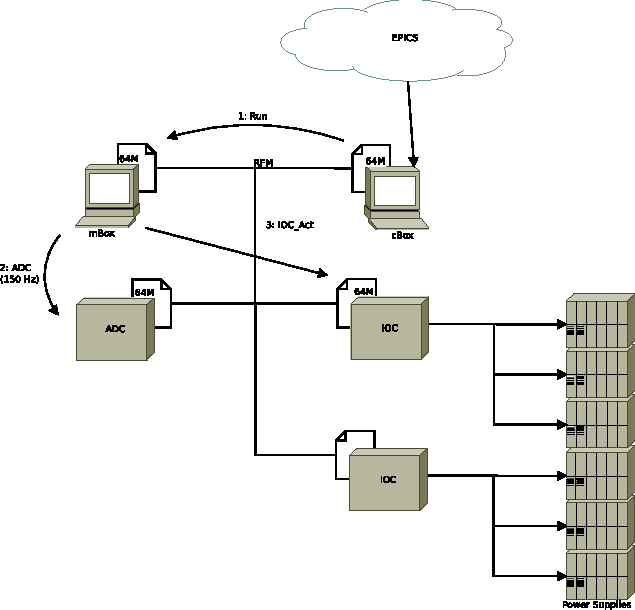
\includegraphics[width=.85\linewidth]{img/mBox_cBox}
    \caption{\label{fig:cbox_mbox}cBox and mBox: the correction infrastructure in BESSY II}
\end{figure}

All elements are connected to a reflective memory (RFM), which provides a high speed and low latency interface. This memory space is split in specified divisions to prevent data collisions.

Two main processes are operating:
\begin{itemize}
    \item the \textbf{cBox} which controls (= \textit{c}) the correction. It defines when to read the values of the BPMs and when to write the new correction values, it provides initializations values. The operators are communicating with this process to configure the correction.
    \item the \textbf{mBox} which does the math (= \textit{m}) of the correction. When allowed by the cBox, it reads the BPMs values, do the maths to define the new correction values and write them to the communication bus. This process also publish the values it reads and write so that client programs can subscribe to this data stream and reuse the values internally.
\end{itemize}

After having received the command to run from the cBox, the mBox queries the ADC (Analog-to-Digital Converter) to provide the BPM values in the RFM. The correction is then calculated (in Amperes) and the values are converted in a format easily transmissible. This data is written back to RFM and read by the IOCs (Input-Output Controllers) that relay to the power supplies alimenting the corrector magnets.

The full process is repeated at a frequency of 150~Hz. 

\section{Improvement of the correction of harmonic perturbations}
\subsection{Acquisition of the frequency-dependent response matrix}
\subsection{Correction of harmonic perturbations}

\renewcommand\cftappendixname{\appendixname~}
%%
%  Bibliography
%%
\bibliographystyle{IEEEtran}
\bibliography{biblio}

\appendix
\renewcommand{\appendixname}{}
%\appendixpage
\makeatletter
\titleformat{\chapter}{\bfseries\Huge}{}{0ex}{}
\makeatother
\chapter{Appendices}
% !TeX encoding = UTF-8
% !TeX spellcheck = en_US
% !TeX root = main.tex

\section{Brightness and brilliance}
\label{apx:brightness_brilliance}
In the following section, the $\theta$ subscript is either $x$ or $y$.

The quality of the beam is described by the \emph{brightness} and the \emph{brilliance}.

Let F be the \emph{flux} of photons, normalized to a beam current of 1~A
\begin{equation}
F = \frac{\text{photons}}{\text{s 0.1\% BW A}},
\end{equation}

The brightness describes the angular divergence of the beam (given by $\sigma_\theta'=\sqrt{\frac{\varepsilon_\theta}{\beta_\theta}}$). It is defined as:
\begin{equation}
S = \frac{F}{2 \pi \sigma'_x \sigma'_y} = \frac{F \sqrt{\beta_x \beta_y}}{2 \pi \sqrt{\varepsilon_x \varepsilon_y}} = \frac{\text{photons}}{\text{s 0.1\% BW mrad$^2$ A}}
\end{equation}
while the brilliance includes also the transverse dimensions ($\sigma_\theta=\sqrt{\varepsilon_\theta \beta_\theta}$):
\begin{equation}
B = \frac{F}{4 \pi^2 \sigma_x \sigma_y \sigma'_x \sigma'_y} = \frac{F}{4 \pi^2 \varepsilon_x \varepsilon_y} = \frac{\text{photons}}{\text{s 0.1\% mm$^2$ BW mrad$^2$ A}}
\end{equation}

These definitions vary in literature. These are taken from the book of K.~Wille~\cite{book:wille}, and apply to Gaussian-shaped electron beams. The invariant idea is that both values are determinated by the beam emittance $\sigma$: the design of the accelerators and the correction are aimed at obtaining the smallest emittance $\varepsilon_\theta$ as possible.

\section{Principal components analysis -- Karhunen-Loève transform (KLT)}
\label{apx:KLT}

Let $\mat{X}$ be a signal with n dimensions.

\begin{equation}
\mat{X} = \left[
\begin{array}{@{}c|c|c|c@{}}
&&&\\ \vec{X}_1 & \vec{X}_2 & \dots & \vec{X}_n \\ &&&
\end{array}
\right]
\end{equation} 

The covariance matrix is extracted
\begin{equation}
\mat{A} = \text{covar}(X) 
\end{equation}
and diagonalized so that the eigenvalues are sorted in a decreasing order (the first one being the most significant). The covariance being symmetric, it is always diagonalizable in $\mathbb{R}$.
\begin{equation}
\mat{D} = \mat{P}^{t} \mat{A} \, \mat{P} 
\end{equation}

The principal components are 
\begin{equation}
\hat{\mat{X}} = \mat{P}^{t} \mat{X}
\end{equation}
and in the first column of the matrix is the most significant one.


\end{document}

